Measurements of $x_{1} = \text{stiffness}$ and $x_{2} = \text{bending strength}$ for a sample of $n = 30$ pieces
of a particular grade of lumber are given in Tobie 5.11. The units are $\text{pounds}/{(\text{inches})}^{2}$.
Using the data in the table,

\begin{enumerate}[label= (\alph*)]
    \item Construct and sketch a 95\% confidence ellipse for the pair ${[\mu_{1}, \mu_{2}]}^{\prime}$, where $\mu_{1} = E(X_{1})$ and $\mu_{2} = E(X_{2})$.

    \begin{figure}[H]
        \centering
        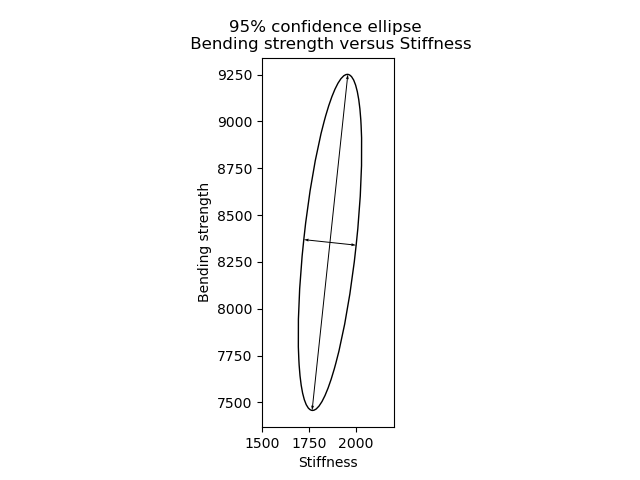
\includegraphics[scale=0.75]{./python/chapter-5/Question-5-19-a.png}
    \end{figure}

    \item Suppose $\mu_{10} = 2000$ and $\mu_{20} = 10,000$ represent ``typical'' values for stiffness and
    bending strength, respectively. Given the result in (a), are the data in Table 5.11 consistent
    with these values? Explain.

    \begin{figure}[H]
        \centering
        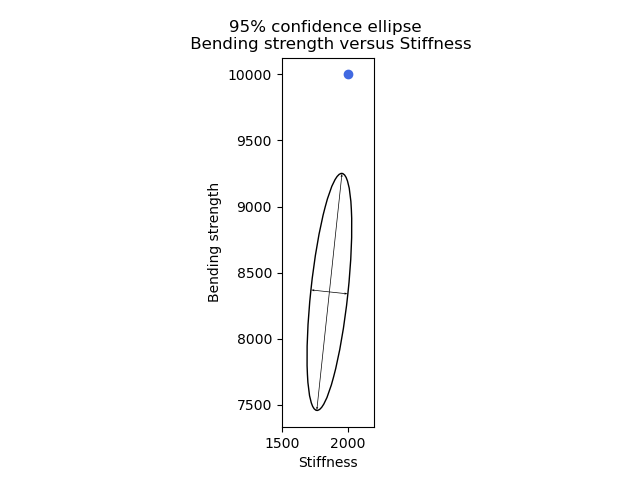
\includegraphics[scale=0.75]{./python/chapter-5/Question-5-19-b.png}
    \end{figure}

    No, the plot above illustrates that the point $[2000, 10000]$ is outside the confidence region defined in part (a), so the values are not consistent with the data. More specifically, the stiffness value of $\mu_{10} = 2000$ is within the bounds, but the bending strength value of $\mu_{20} = 10,000$ is way too big.

    \item Is the bivariate normal distribution a viable population model? Explain with reference to \textit{Q-Q} plots and a scatter diagram.
    
    \begin{figure}[H]
        \centering
        \begin{tabular}{cc}
            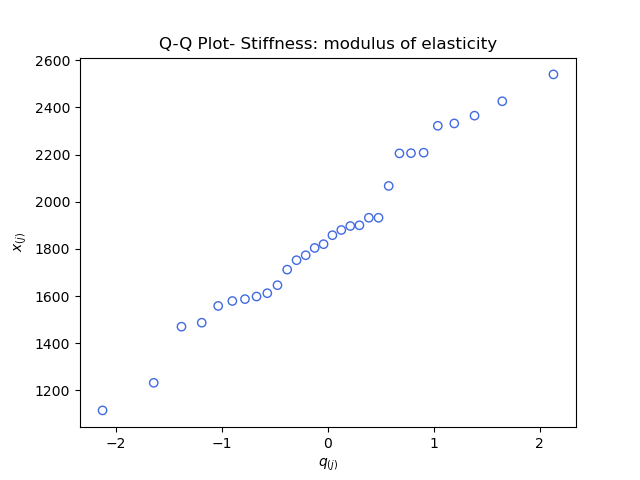
\includegraphics[scale=0.35]{./python/chapter-5/Question-5-19-c-QQ-Stiffness.png} &
            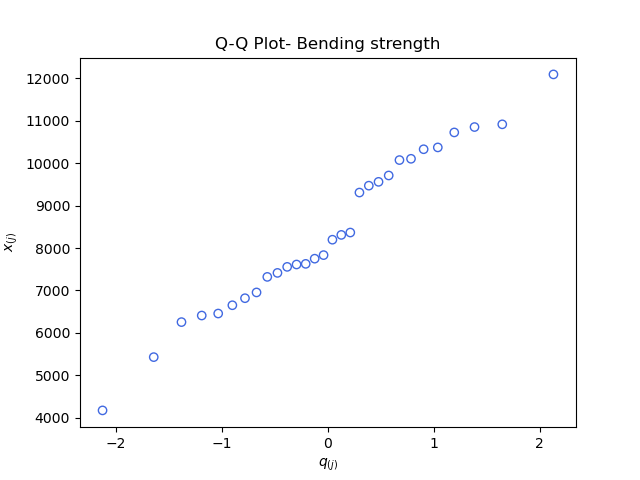
\includegraphics[scale=0.35]{./python/chapter-5/Question-5-19-c-QQ-Bending.png}
        \end{tabular}
    \end{figure}

    \begin{figure}[H]
        \centering
        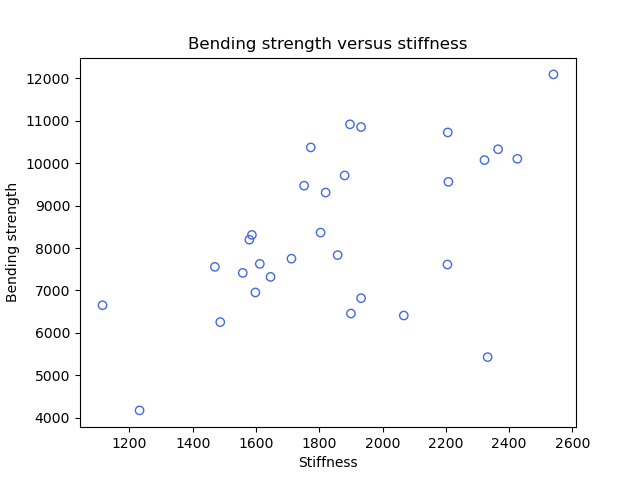
\includegraphics[scale=0.55]{./python/chapter-5/Question-5-19-c-xy.png}
    \end{figure}
\end{enumerate}

The \textit{Q-Q} plots for stiffness and bending strength, both appear to be linear. There are some jumps in values, but overall look okay, so the data is univariate normal. The scatterplot of the data doesn't appear to have a strong linear trend, but the data are mostly grouped together. I would say the data is roughly birvariate-normal. A $\chi^{2}$-plot, not shown here, does identify a few outliers.